\documentclass[11pt]{article}
    \title{\textbf{AI Project 3 Report}}
    \author{Tobias Dault, Eyob Tekle, William Thomson Jr.}
    \date{1 April 2022}
    
    \addtolength{\topmargin}{-4cm}
    \addtolength{\textheight}{3cm}
\usepackage{graphicx}
\graphicspath{ {./assets/} }
\begin{document}

\maketitle
\thispagestyle{empty}

\section{Introduction}
The purpose of our program is to collect names of attributes, values of attributes, hard constraints, and preferences for the reason of performing four reasoning tasks: Existence of feasible objects, exemplification, optimization, and omni-optimization.
\\\\\\\\\\\\

\section{How it works}
Using a GUI written in Python (using Tkinter framework), input is taken through either the text input boxes or file input buttons.
\begin{description}
\addtolength{\itemindent}{0.80cm}
\itemsep0em
\item[Binary Attributes] Step 1: Follow steps in the README to start the program\\
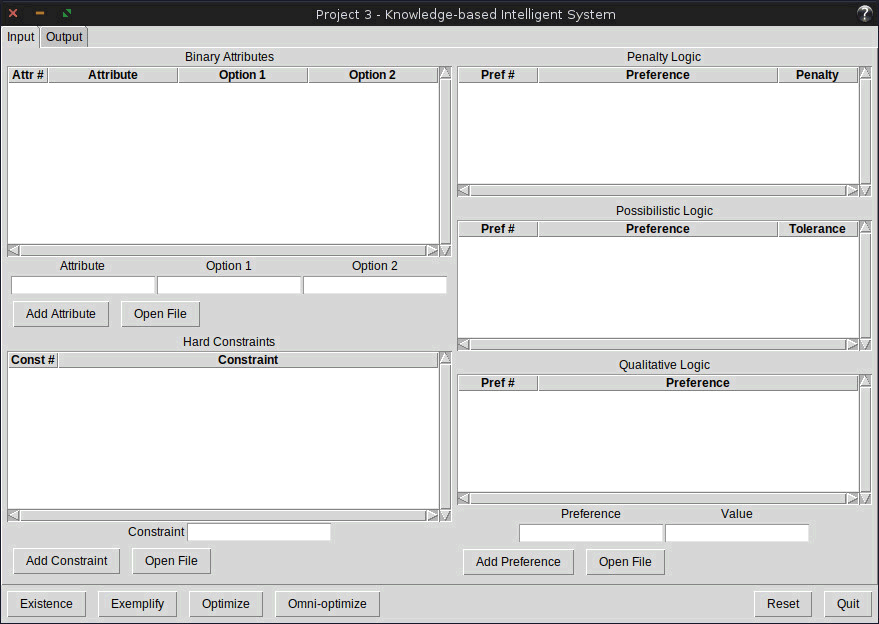
\includegraphics[scale=0.3]{input_start} \\\\
Step 2: Click the "Open File" button under Binary Attributes\\
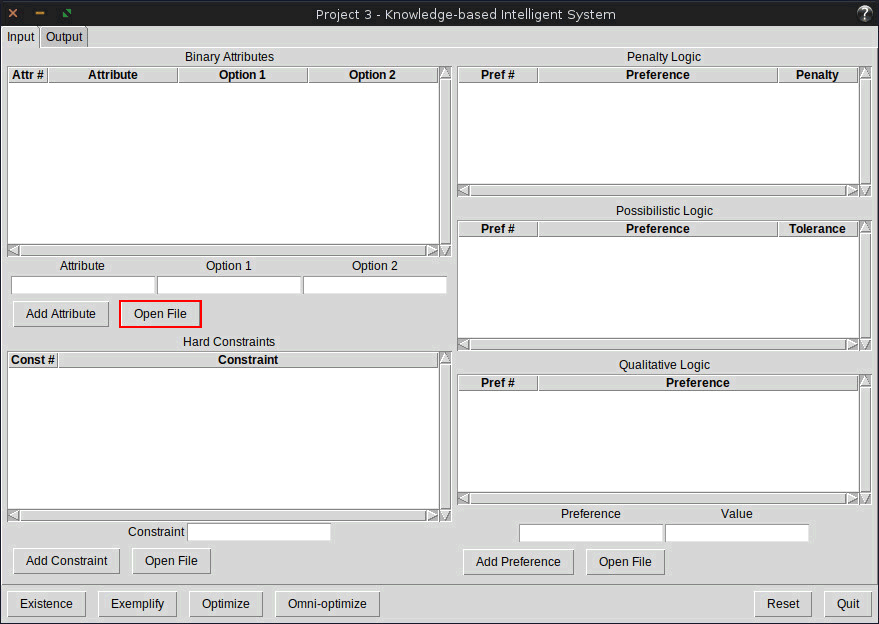
\includegraphics[scale=0.3]{input_attributes}\\
Step 3: Select your desired file (attributes$\_$test.txt for this example) and click "Open".\\
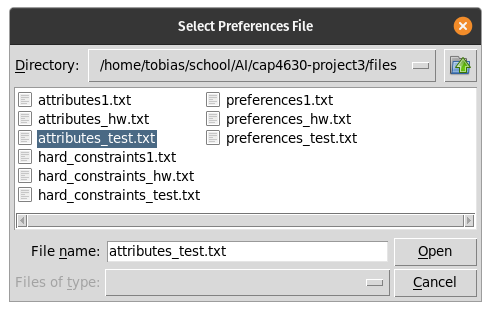
\includegraphics[scale=0.3]{select_attributes}\\
The contents of the file will be displayed under Binary Attributes.\\
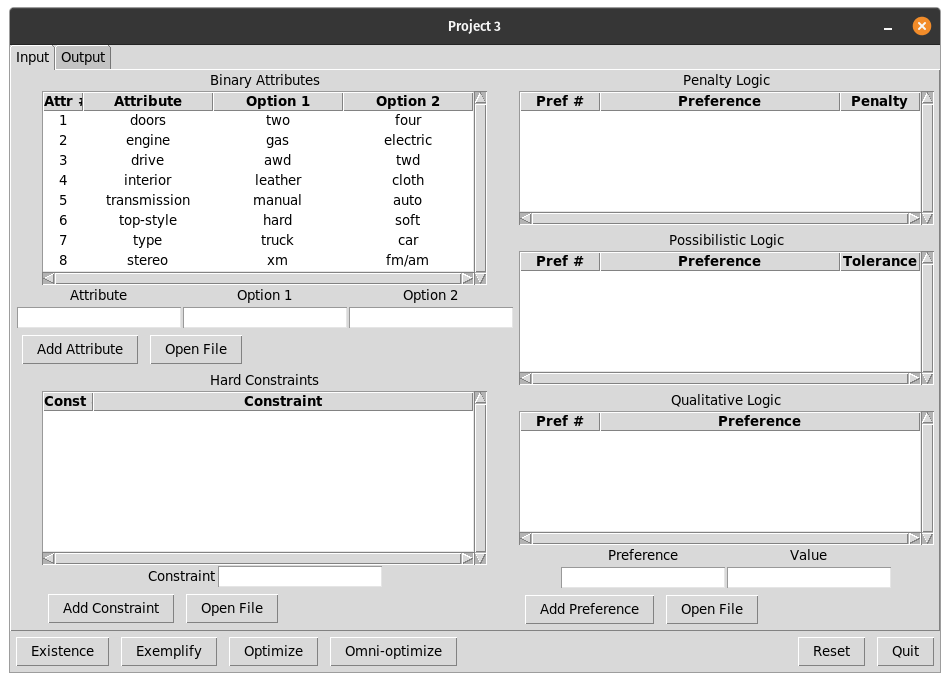
\includegraphics[scale=0.3]{attributes_imported}\\\\\\

\item[Hard Constraints] Step 1: Click the "Open File" button under Hard Constraints\\
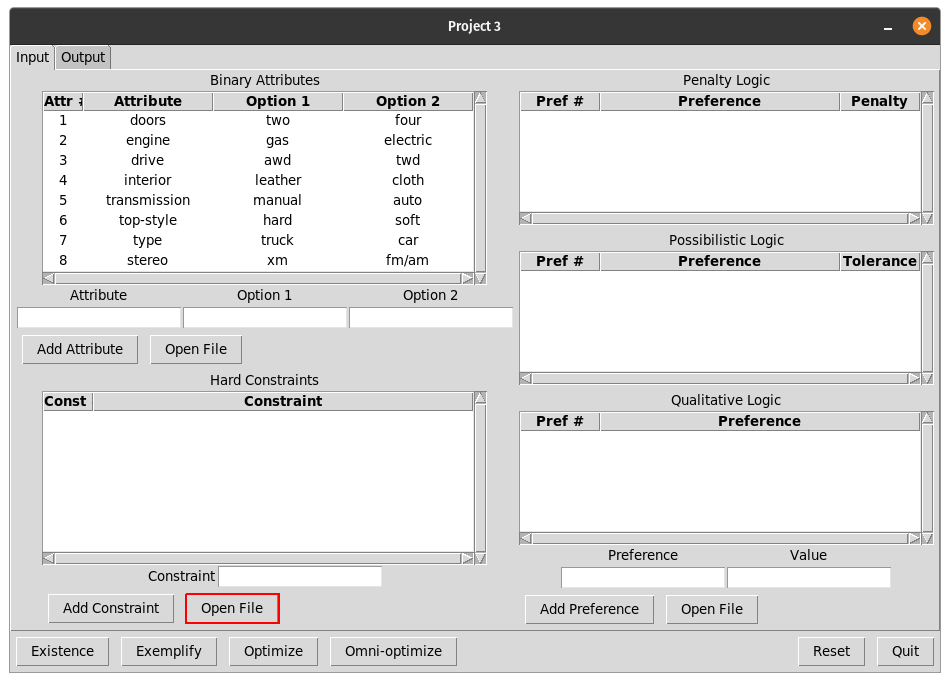
\includegraphics[scale=0.3]{input_constraints} \\\\
Step 2: Select your desired file (hard$\_$constraints$\_$test.txt for this example) and click "Open".\\
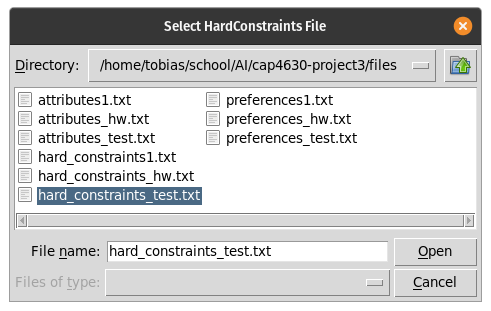
\includegraphics[scale=0.3]{select_constraints}\\
Step 3: The contents of the file will be displayed under Hard Constraints.\\
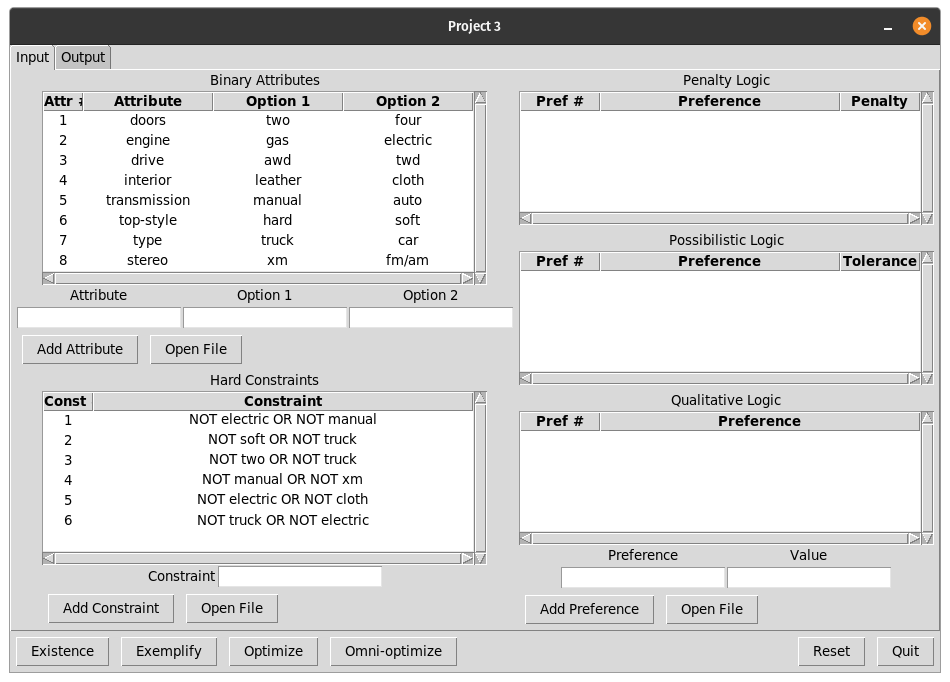
\includegraphics[scale=0.3]{constraints_imported}\\

\item[Logics] Step 1: Click the "Open File" button under the three logics\\
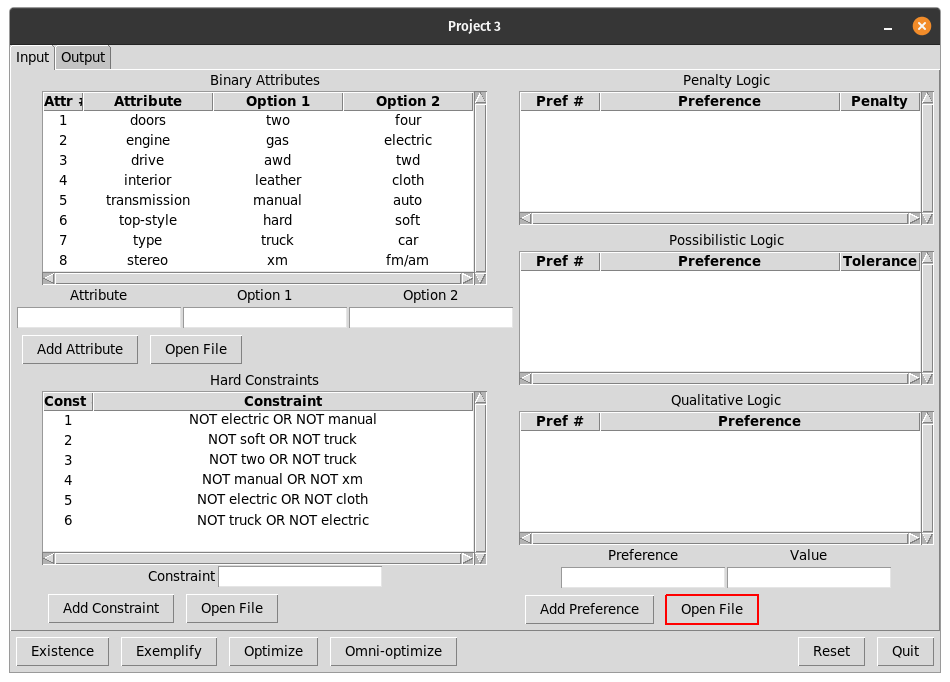
\includegraphics[scale=0.3]{input_preferences} \\\\
Step 2: Select your desired file (preferences$\_$test.txt for this example) and click "Open".\\
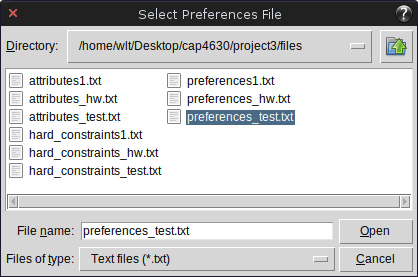
\includegraphics[scale=0.3]{select_preferences}\\
Step 3: The contents of the file will be displayed in the three.\\
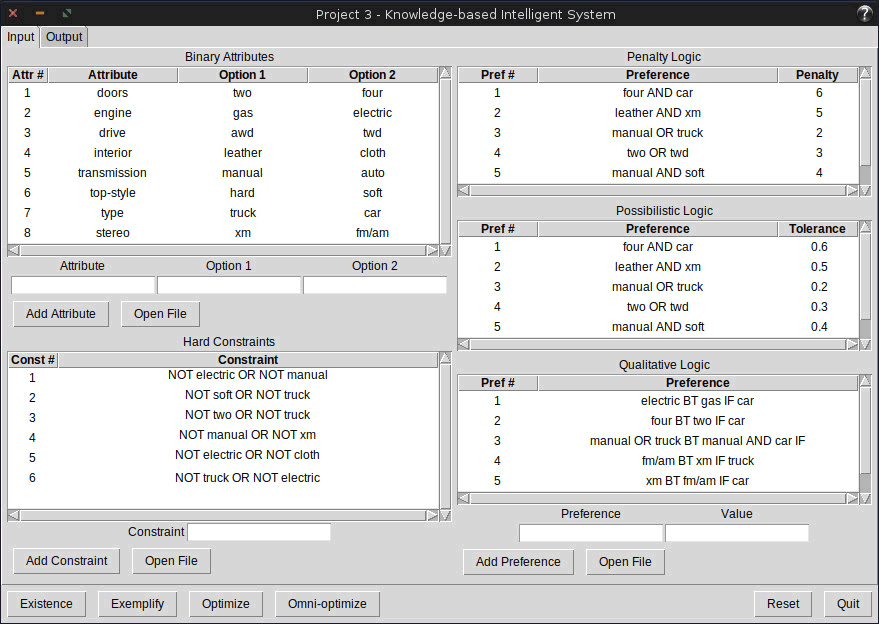
\includegraphics[scale=0.3]{preferences_imported}\\\\\\\\\\


\item[Existence of Feasible Objects] Step 1:\\
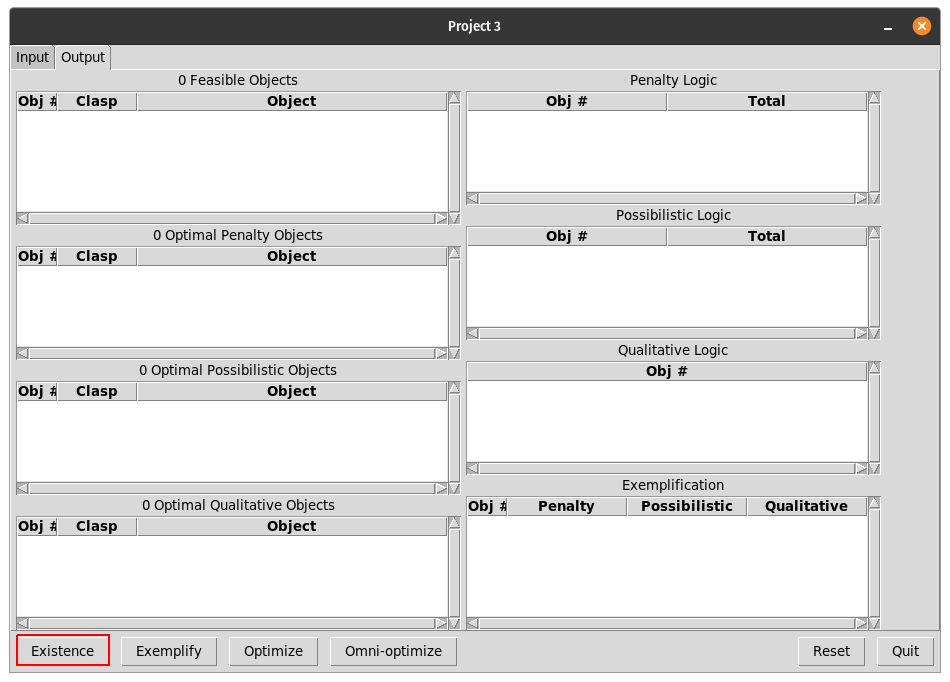
\includegraphics[scale=0.3]{existence}
\end{description}

\section{Examples}
Using the three text files provided in cap4630-project3/files (attributes$\_$test.txt, hard$\_$constraints.txt, preferences$\_$test.txt), here is an example of getting results using the test instance.


\end{document}